%%%% SemDial Proceedings template by Raquel Fernández, 2013.
%%%% Modified by Simon Dobnik for the proceedings of IWCS 2019.
%%%% Modified by Yannick Parmentier and Sylvain Pogodalla for the proceedings of TALN 2020.

\documentclass[a4paper,11pt,oneside,english]{book}

\usepackage{times}
\usepackage[a4paper,hmargin=1.2cm,top=1cm,bottom=2.5cm, includefoot=true, hcentering]{geometry}

\setlength{\parindent}{0pt}

\usepackage[english]{babel}
\usepackage[num]{isodate}
\usepackage[utf8]{inputenc} 
\usepackage[T1]{fontenc} % fonts to encode unicode
\usepackage{changepage}  % for local redefinition of margins
\selectlanguage{UKenglish}

\usepackage{wallpaper} %for image on frontpage

\usepackage{tabularx}
\usepackage{tipa} 
\usepackage{newunicodechar}
\newunicodechar{ʁ}{\textipa{K}}
\newunicodechar{ʒ}{\textipa{Z}}
\newunicodechar{ʃ}{\textipa{S}}

\newif\ifbackground
BACKGROUND-PLACEHOLDER
\newif\iflogo
LOGO-PLACEHOLDER
\newif\ifcredits
CREDITS-PLACEHOLDER
\newif\ifsponsors
SPONSORS-PLACEHOLDER
\newif\ifmessage
MESSAGE-PLACEHOLDER
\newif\ifpreface
PREFACE-PLACEHOLDER
\newif\ifcommittee
COMMITTEE-PLACEHOLDER
\newif\ifinvited
INVITED-PLACEHOLDER

\usepackage{xspace}
\usepackage{url}
\usepackage{tikz}

\usepackage{ragged2e}
\usepackage{tcolorbox}

\usepackage{pdfpages}
\usepackage{pax}

\usepackage[newparttoc]{titlesec}
\titleformat{\part}[display]{\center\normalfont\huge\bfseries}
            {\partname\ \thepart}{20pt}{\Huge} 

\usepackage{etoolbox}
\usepackage[colorlinks,
            allcolors=blue!60!black,
            breaklinks=true,
            %%% EDIT TITLE: %%%
            pdftitle={ABBREV-PLACEHOLDER},
           ]{hyperref}   % hyperlinked table of contents, etc.

\newcounter{article}
\newcounter{articlePage}[article]

\def\oldsession{}
\def\cursession{SESSION-PLACEHOLDER}

\usepackage{pdftexcmds}
\makeatletter
\newcommand\comparesessions[3]{%
  \ifnum\pdf@strcmp{#1}{#2}=0 %
     \expandafter\@firstoftwo
  \else
    \expandafter\@secondoftwo
  \fi
    {}
    {\atoc{#3}}%
}
\makeatother

\newcommand{\atoc}[1]{%
  \part{#1}%
}

\def\halid{hal-0001}
\newcommand\HAL[1]{\ifstrempty{#1}{}{\textsc{hal}~: \href{https://hal.archives-ouvertes.fr/#1}{#1}}}

\usepackage{fancyhdr}

\newlength{\HeaderHeight}
\newsavebox{\HeaderBox}
\savebox{\HeaderBox}{%
  \small
  \slshape
  \begin{tabular}{@{}p{\textwidth}}
    BOOK-PLACEHOLDER\\
    LOCATION-PLACEHOLDER, DATE-PLACEHOLDER
  \end{tabular}}

\settoheight{\HeaderHeight}{\usebox{\HeaderBox}}

\setlength{\headheight}{\HeaderHeight}
\setlength{\headheight}{61pt}

\fancyhf{}
\fancyhead[L]{%
  \ifnumequal{\value{articlePage}}{1}{%
    \numdef{\lastpage}{\thepage + \lastbutonepage}
    {\usebox{\HeaderBox}}{}}%
}
\renewcommand{\headrulewidth}{0pt}
\fancyfoot[C]{%
  \ifnumequal{\value{articlePage}}{1}{%
    \numdef{\lastpage}{\thepage + \lastbutonepage}
    {\small
      \begin{tabular}{l}
        TRACK-NAME-PLACEHOLDER, pages \thepage--\lastpage.\\%
        \ifthenelse{\equal{\halid}{}}{}{\ifthenelse{\equal{HAL-PLACEHOLDER}{}}{}{HAL-PLACEHOLDER.\\}}         
        \includegraphics[height=10pt]{by.eps}
        \href{http://creativecommons.org/licenses/by/4.0/}{Attribution 4.0 International}.
  \end{tabular}}}{\thepage}%
}

\pagestyle{plain}

% Parameters: file name, title, authors, horizontal offset, vertical offset
\newcommand{\paper}[7]{%
\cleardoublepage

\def\cursession{#7}
\ifthenelse{\equal{\cursession}{}}{}{%
  \comparesessions{\oldsession}{\cursession}{#7}
}

\phantomsection
\addcontentsline{toc}{chapter}{#2}%
\addtocontents{toc}{$\,$\textit{#3}\par}%

\edef\oldsession{\cursession}

\pdfximage{#1}% Read entire PDF
\edef\totalpages{\the\pdflastximagepages}% Store number of pages
\edef\lastbutonepage{\number\numexpr\totalpages-1}% Store last page - 1
\refstepcounter{article}
\def\halid{#6}
\includepdf[pages=-,width=\textwidth,offset={#4 #5},pagecommand={\pagestyle{fancy}\refstepcounter{articlePage}}]{#1}
\cleardoublepage}

\newcommand{\goodpaper}[5]{\paper{#1}{#2}{#3}{-0mm}{-0mm}{#4}{#5}}

%\draft

\usepackage{lmodern}
\ifpdf
\usepackage{pdfcolmk}
\fi
%% check if using xelatex rather than pdflatex
\ifxetex
\usepackage{fontspec}
\fi
\usepackage{graphicx}
%% drawing package
\usepackage{tikz}
%% for dingbats
\usepackage{pifont}
\providecommand{\HUGE}{\Huge}% if not using memoir
\newlength{\drop}% for convenience
%% publisher's logo
\newcommand*{\plogo}{%
  
\includegraphics[width=.3\textwidth]{logo.png}
}

\newcommand*{\titleUL}{\begingroup%
  \drop=0.1\textheight
  \vspace*{\drop}
  \begin{center}
    {\LARGE \textsc{~~~~~}}\\[\drop]
    \iflogo
        {\LARGE \plogo}\\[2ex]
    \fi
    \rule{\textwidth}{1pt}\par
    \vspace{0.5\baselineskip}
    {\Large\bfseries \textsl{TITLE-PLACEHOLDER} \\(ABBREV-PLACEHOLDER)\footnote{\url{URL-PLACEHOLDER}}\\[2ex]
      \large BOOK-PLACEHOLDER. \\[1ex]
      \large TRACK-NAME-PLACEHOLDER}\\[2ex]
    \rule{\textwidth}{1pt}\par
    \vspace{1ex}
    \vfill
    CHAIRS-PLACEHOLDER (\'Eds.) 
    \vfill
    LOCATION-PLACEHOLDER, DATE-PLACEHOLDER \\[1ex]
  \end{center}
\endgroup}

\usepackage{bookmark}

\begin{document}

\titleUL

\renewcommand{\headrulewidth}{0pt}
\renewcommand{\footrulewidth}{0pt}

\pagenumbering{roman}
%%  TITLE PAGE 
%%%%%%%%%%%%%%%%%%%%%%%%%%%%%%%%%%%%%%%%%%%%%%%%%%%%%%%%%%%%%%%%%%%%%%%%%%%%%%%%
\pdfbookmark{TITLE-PLACEHOLDER}{title}
\thispagestyle{empty}

\ifbackground
%\tikz[remember picture,overlay] \node[opacity=0.7,inner sep=0pt] at (current page.north){
\includegraphics[width=\paperwidth,height=.5\paperheight]{background}};
\ThisULCornerWallPaper{1}{background.png}
\fi

\clearpage

%%%% Crédits et copyright
\thispagestyle{empty}
\mbox{}
\vfill
\ifcredits
\input{credits.tex}

\fi
\large
\noindent
\copyright YEAR-PLACEHOLDER PUBLISHER-PLACEHOLDER 
\hspace*{6.5mm} \\

\clearpage

%% DETAILS 
%%%%%%%%%%%%%%%%%%%%%%%%%%%%%%%%%%%%%%%%%%%%%%%%%%%%%%%%%%%%%%%%%%%%%%%%%%%%%%%
\pdfbookmark{ISBN}{isbn}
\thispagestyle{empty}

\ifsponsors
\section*{Sponsors}
\vspace*{0.5cm}

% SPONSOR LOGOS
\begin{center}
\includegraphics[width=.8\textwidth]{sponsors.png}
\end{center}
\fi

\clearpage

%%%%%%%%%%%%%%%%%%%%%%%%%%%%%%%%%%%%%%%%%%%%%%%%%%%%%%%%%%%%%%%%%%%%%%%%%%%%%%%%%%%%%%%%%%%%%%% 
\ifmessage
\pdfbookmark{Message}{message}

\input{message.tex}

\clearpage
\fi
%%%%%%%%%%%%%%%%%%%%%%%%%%%%%%%%%%%%%%%%%%%%%%%%%%%%%%%%%%%%%%%%%%%%%%%%%%%%%%%%%%%%%%%%%%%%%%% 
\ifpreface
\pdfbookmark{Preface}{preface}

\section*{Preface}
\vspace*{0.5cm}

\input{preface.tex}

\clearpage
\fi
%%%%%%%%%%%%%%%%%%%%%%%%%%%%%%%%%%%%%%%%%%%%%%%%%%%%%%%%%%%%%%%%%%%%%%%%%%%%%%%%%%%%%%%%%%%%%%% 
\ifcommittee
\pdfbookmark{Committees}{pc}

\section*{Committees}
\vspace*{0.5cm}

\input{committee.tex}

\clearpage
\fi
%%%%%%%%%%%%%%%%%%%%%%%%%%%%%%%%%%%%%%%%%%%%%%%%%%%%%%%%%%%%%%%%%%%%%%%%%%%%%%%%%%%%%%%%%%%%%%%
\ifinvited
\pdfbookmark{Invited talks}{invited}

\section*{Invited talks}
\vspace*{0.5cm}

\input{invited.tex}

\clearpage
\fi
%%%%%%%%%%%%%%%%%%%%%%%%%%%%%%%%%%%%%%%%%%%%%%%%%%%%%%%%%%%%%%%%%%%%%%%%%%%%%%%%%%%%%%%%%%%%%%%


\pdfbookmark{Table of contents}{toc}
\setlength{\parskip}{0pt}

\renewcommand{\contentsname}{\mbox{}\\[-108pt]\noindent\textbf{\Large
    Table of contents}\\[-28pt]}
\tableofcontents
\cleardoublepage

\bookmark[dest=dummy,level=1]{EndofFrontmatter}
\hypertarget{dummy}{}

\pagenumbering{arabic}
%%%%%%%%%%%%%%%%%%%%%%%%%%%%%%%%%%%%%%%%%%%%%%%%%%%%%%%%%%%%%%%%%%%%%%%%%%%%%%%%%%%%%%%%%%%%%%%
\pagestyle{fancy}

\setcounter{page}{PAGE-PLACEHOLDER} %% used for backward compatibility
                                    %% (page numbers of handcrafted proceedings) 
\include{all_papers}


%%%%%%%%%%%%%%%%%%%%%%%%%%%%%%%%%%%%%%%%%%%%%%%%%%%%%%%%%%%%%%%%%%%%%%%%%%%%%%%%%%%%%%%%%%%%%%%
\clearpage
\thispagestyle{empty}
\mbox{}

\end{document}
